\subsection{Implementation}
Our framework is implemented with Pytorch. We used AES-CFB-128 as the authenticated encryption algorithm as Bonawitz \emph{et al}. did~\cite{Practical}. We adopted MNIST and CIFAR-10 as datasets, which are also used in the original FedAvg~\cite{mcmahan2016communicationefficient}. We trained a simple convolutional neural network for the classification task. Our experiments are carried on a PC with an Intel i7-8700 CPU (3.2GHz), 16 GB of RAM, and a GTX 1080 GPU. The model was executed in a single thread to facilitate comparing and analyzing. The optimizer was stochastic gradient descent (SGD) and the learning rate is $0.01$. The $fraction$ is set as $0.1$ which means that $10\%$ of clients will be chosen to carry on the training process in each epoch. 
% Our demo is open-sourced on \url{https://github.com/Carudy/DemoFL}.

\subsection{Accuracy}
Although our work does not modify the learning module compared to other federated learning frameworks, we still conducted a series of experiments to observe the accuracy. We compared FedAvg with our framework on both independently identically distribution (IID) data and non-IID data to verify the effectivity. Since this experiment aims to prove the validity instead of high accuracy, the models were not trained to obtain high accuracy. We conducted experiments with MNIST in non-IID and CIFAR-10 in IID, and Figure~\ref{acc} shows the result. With IID data, our framework obtains a similar performance compared with FedAvg. With non-IID data, the two systems did not match as well as they were with IID data when the $epoch$ was small. However, they finally converged to the same stable scope with the same speed, which confirmed the differences were caused by biases. Therefore, our framework can achieve the same learning goal as FedAvg while providing privacy guarantees and system robustness.

\begin{figure}[!ht]
    \centering
    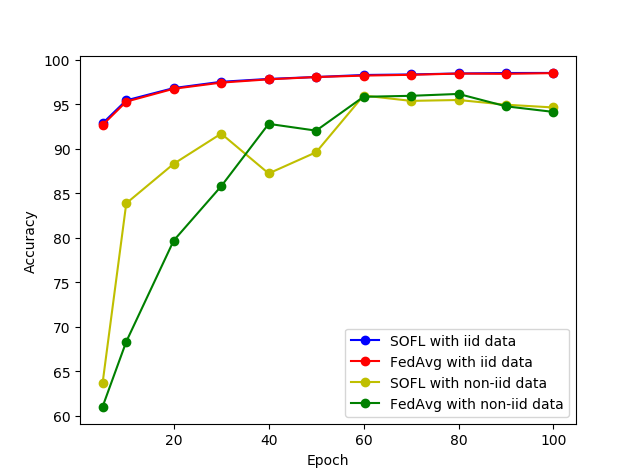
\includegraphics[width=\columnwidth]{img/acc.png}
    \caption{The accuracy of FedAvg~\cite{mcmahan2016communicationefficient} and DemoFL with IID data from CIFAR-10, and non-IID data from MNIST. The horizontal axis $epoch$ means the total rounds that the federated learning system has been trained for. }
    \label{acc}
\end{figure}

\begin{figure}[!ht]
    \centering
    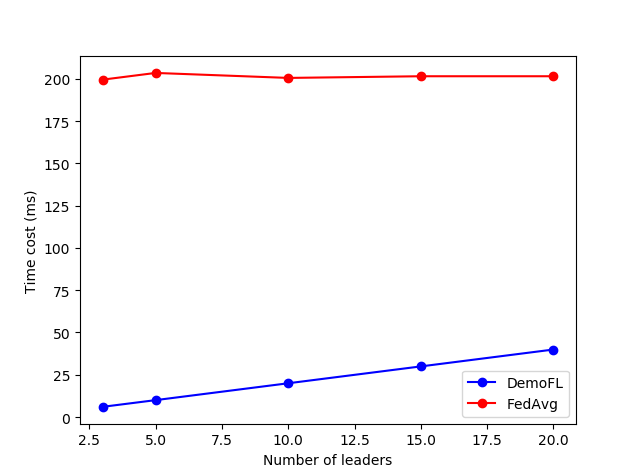
\includegraphics[width=\columnwidth]{img/leader-time.png}
    \caption{The average time spent on computation in set-up process DemoFL VS different proportions of leaders.}
    \label{leader-time}
\end{figure}

\subsection{Set-up Overhead}
In the set-up phase, our system selects several clients as leaders, and the number of leaders impacts the efficiency and a particular leader's load because a common user needs to build secure communication channels with all leaders. To discover the relation between the number of leaders and the computation overhead, we set the number of clients on different levels and conducted experiments with different numbers of leaders. Figure~\ref{leader-time} shows the linear relationship between each user's computation time spent on Diffie Hellman key-exchange protocol and the number of leaders. The overhead of time in the set-up process is also very low because DemoFL has no complex calculations as Bonawitz \emph{et al}.~\cite{Practical}'s secure aggregation scheme does. In Bonawitz's scheme, participants need to calculate secret keys for all other users and generate t-out-of-n secret shares for the pseudorandom generator (PRG) seed and their secret keys. The comparison is illustrated in Figure~\ref{avg-user-cpu}. Since Bonawitz's scheme has a time complexity of $O(n^2)$, the computation overhead of it is much higher than DemoFL. Method of Kanagavelu \emph{et al}.~\cite{Two-Phase} performs the same as Bonawitz's scheme because they also have an $O(n^2)$ set-up. Therefore, employing fewer leaders can help to improve efficiency, and in contrast, employing more leaders can are beneficial to security because a successful attack requires all leaders compromised. 

Meanwhile, with more leaders, one common user needs to store more keys for leaders. Apparently, the relationship between the number of leaders and one user's storage overhead is also linear. However, in Bonawitz's scheme, a client needs to storge two t-out-of-n secret shares for all others. The storage complexity of DemoFL and Bonawitz's scheme is $O(N_l)$ and $O(n)$ respectively, where $N_l \ll n$. Therefore, DemoFL has a very trivial set-up overhead on both time and storage, which is friendly to individual participants such as smartphones.

\begin{figure}[!ht]
    \centering
    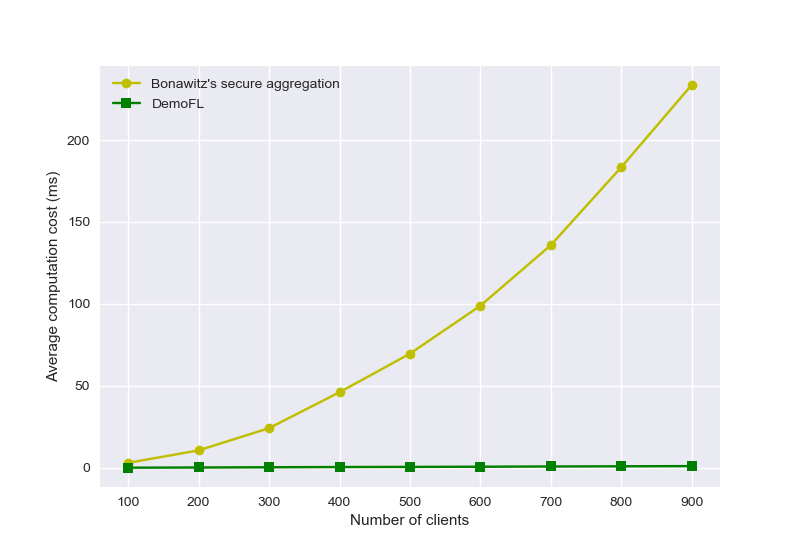
\includegraphics[width=\columnwidth]{img/avg-user-cpu.png}
    \caption{The average time spent on computation in set-up process of Bonawitz's secure aggregation~\cite{Practical} and DemoFL VS the number of clients. The proportion of leaders is set to $3\%$.}
    \label{avg-user-cpu}
\end{figure}

\subsection{Efficiency}
Our framework primarily addresses the server-based situation, where a participant's computing capability is far weaker than the server. And for the server, the overhead of computations such as MPC is insignificant compared to the communication overhead because of its powerful computing capability. Therefore, we carried out experiments to evaluate the computation overheads for participants only, and communication overheads for both participants and servers in DemoFL and Bonawitz's secure aggregation scheme. Experiments in this subsection are with the assumption that there are no dropouts or crashes.

To evaluate the computation overheads, we fixed the number of clients to 100 and the proportion of leaders to $3$ and tested the average running time of a single participant. In DemoFL, participants are divided into two categories: common users and leaders, and a participant can hold both identities at the same time. While in Bonawitz's secure aggregation scheme, all users are treated equally. The result is displayed in Figure~\ref{learning-overhead}. It suggests that participants of DemoFL have obvious advantages on computation overhead. The reason is that participants of Bonawitz's secure aggregation scheme need to carry out more encryptions/decryptions for unmasking.

Measuring the communication overheads with wall clock time is difficult because it has biases large enough to mislead the judgment. Therefore, we evaluate the communication overhead with the number of communications. We conducted experiments to count up the communications and tried to compare the overheads of DemoFL and Bonawitz's secure aggregation scheme. Since there are no dropouts or crashes, the number of communications in each epoch is fixed. Therefore, we computed the ratio of overheads of Bonawitz's secure aggregation scheme and DemoFL with the number of clients set as $100$ and the number of leaders as $3$, and the result is $1.184$. And if the number of leaders gets larger, this ratio will decrease towards $1$. Since the number of leaders will never be set too large, the communication overhead of DemoFL is advantageous.

\begin{figure}[!ht]
    \centering
    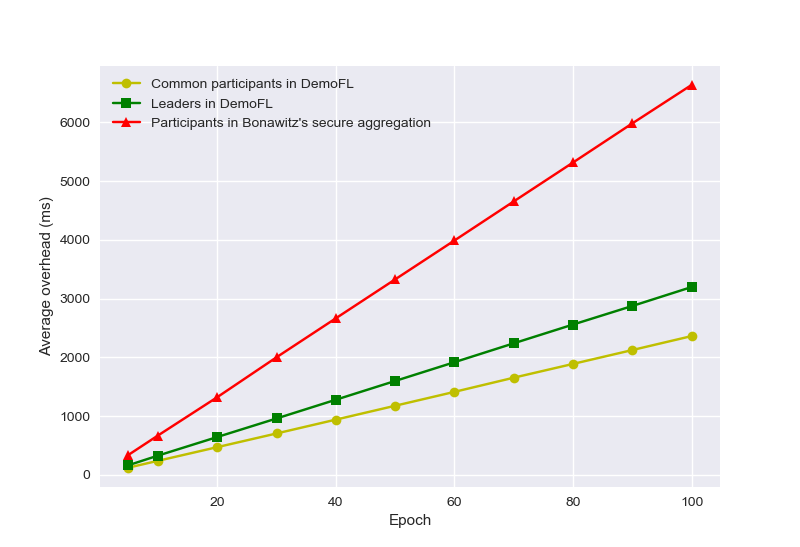
\includegraphics[width=\columnwidth]{img/learning-overhead.png}
    \caption{The average running time per participant in the learning process VS epoch. Without dropouts and reorganization processes.}
    \label{learning-overhead}
\end{figure}

\subsection{Robustness}
\subsubsection{Crash}
The robustness of DemoFL is mainly based on the reorganizing process, which happens when a leader is crashed. We discuss crashes for leaders because a crash of a common user is equivalent to a dropout. Crashes can hardly be completely avoided, therefore, we introduced $crash\_rate$, which is the possibility for each leader that it would crash during one epoch, to help to measure the robustness. Generally, we consider $crash\_rate$ is quite small because compared to dropouts, crashes rarely happen in nowadays smart devices/servers. Therefore we can consider $crash\_rate$ would not be larger than $10\%$. Since a crash causes a reorganizing process, which helps the system by communications, we still adopt the number of communications to evaluate the extra overhead. We conducted several experiments on how $crash\_rate$ impacts efficiency. First, we set the number of clients to 100 and the $crash\_rate$ to $10\%$, which is the worst case. Then we counted up the number of communications at a situation without crashes. Finally, we counted up communications in other situations with different numbers of clients and different numbers of leaders. We consider the ratio of communications in these situations with the original one as their overheads, and the result is shown in Figure~\ref{crash-leader}. 

\begin{figure}[!ht]
    \centering
    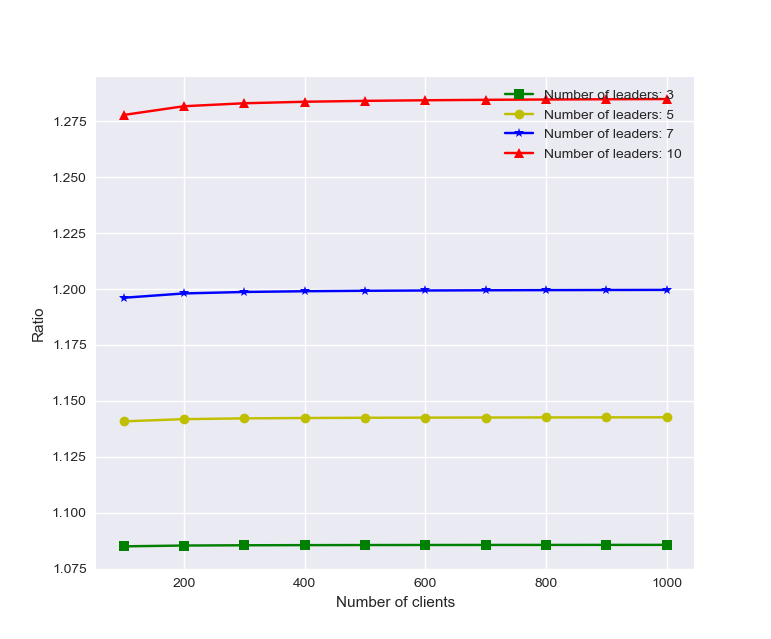
\includegraphics[width=\columnwidth]{img/crash-leader.png}
    \caption{The ratio of communications VS number of clients and leaders.}
    \label{crash-leader}
\end{figure}

The number of clients hardly affects the overheads. In contrast, the number of leaders is very influential. Therefore, we suggest setting the number of leaders as smaller as possible. Generally, $3$ or $5$ could be sufficient choices.

\begin{figure}[!ht]
    \centering
    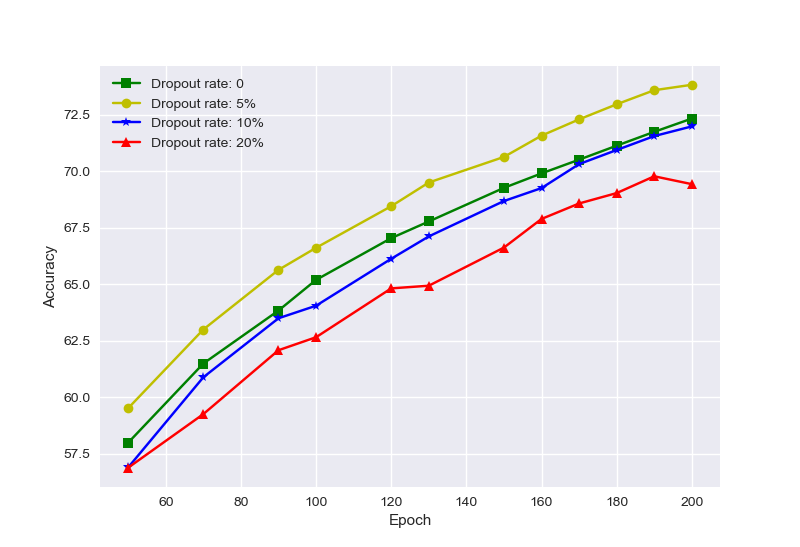
\includegraphics[width=\columnwidth]{img/dropout-acc.png}
    \caption{The accuracy VS different $dropout\_rate$s.}
    \label{dropout-acc}
\end{figure}

\subsubsection{Network Delay and Dropout}
Sometimes several packets cannot be received in time due to network delays or dropouts. Bonawitz \emph{et al}.'s method~\cite{Practical} has considered this issue and it has a ``double-masking'' scheme to address it, which has a high computation overhead. In DemoFL's secure learning process, a leader will not be waiting for participants'parameters permanently. It has a time limit, over which the leader will abandon waiting and send the current $B_j$ to the server (introduced in Section~\ref{sec:DemoFL}). Under this circumstance, some common parties will be recognized as having lost connection and removed from the participant-group without contributing to the learning process. However, if a party does not lose the connection while its message reached the leader late because of network delay, discarding it may influence the target model's accuracy. Since the leaders will compute the intersection no matter there are dropouts or not, the dropouts have no negative effect on efficiency. We set the $dropout\_rate$ to show the probability that a common party fails to send its parameters to leaders due to packet loss or network delay in one epoch. We then carried out several experiments to observe how package losses impact the learning process. The result is shown in Figure~\ref{dropout-acc}. The result indicates that the influence of dropouts on accuracy is acceptable when $dropout\_rate$ is no more than $10\%$: when the $Epoch$ gets larger than about $160$, the accuracy gap between no-dropout models and with-dropout models becomes insignificant. In addition, the accuracy of the model learned in the situation with $5\% dropout\_rate$ is even better than the model learned in the situation without $dropout\_rate$,  which may be caused by biases, or the inherent defects of federated learning's aggregation scheme, and this might be one of our future researches. In summary, DemoFL has a strong resistance to packet loss considering that most machine learning tasks have a large enough $Epoch_{max}$.